\documentclass[11pt,a4paper]{article}

\usepackage[T1]{fontenc}
\usepackage[utf8]{inputenc}
\usepackage{lmodern}
\usepackage[margin=2.4cm]{geometry}
\usepackage{amsmath,amssymb}
\usepackage{booktabs}
\usepackage{xcolor}
\usepackage{listings}
\usepackage{tikz}
\usepackage{enumitem}
\usepackage{microtype}
\sloppy
\usepackage[colorlinks=true,linkcolor=blue!45!black,urlcolor=blue!45!black,
            citecolor=blue!45!black]{hyperref}
\usetikzlibrary{positioning,arrows.meta,fit,backgrounds}

\definecolor{codebg}{RGB}{247,247,244}
\definecolor{codekw}{RGB}{0,80,140}
\definecolor{codecm}{RGB}{110,120,110}
\definecolor{codest}{RGB}{150,60,20}
\definecolor{rule}{RGB}{200,200,195}

\lstset{
  language=Python,
  basicstyle=\ttfamily\footnotesize,
  keywordstyle=\color{codekw}\bfseries,
  commentstyle=\color{codecm}\itshape,
  stringstyle=\color{codest},
  showstringspaces=false,
  backgroundcolor=\color{codebg},
  frame=leftline,
  framerule=0.8pt,
  rulecolor=\color{rule},
  framesep=6pt,
  xleftmargin=10pt,
  breaklines=true,
  breakatwhitespace=true,
  columns=fullflexible,
  keepspaces=true,
  aboveskip=8pt,
  belowskip=8pt,
  numbers=none,
}

\newcommand{\code}[1]{\texttt{\small #1}}
\newcommand{\file}[1]{\texttt{\small #1}}
\newcommand{\eps}{\varepsilon}
\newcommand{\Eg}{E_\gamma}
\newcommand{\BH}{B_{\mathrm{H}}}
\newcommand{\nHI}{n_{\mathrm{H\,I}}}
\newcommand{\sion}{\sigma_{\mathrm{ion}}}
\newcommand{\spi}{\sigma_{\mathrm{pi}}}

\title{\bfseries Block-by-block anatomy of the code that estimates\\
       the number of ionization events per primary electron}
\author{Internal technical note --- Paper 1 (CR electrons during the EoR)}
\date{3 September 2026}

\begin{document}
\maketitle

\begin{abstract}
\noindent
This note documents, block by block, the software that computes
$Y(K_{\mathrm{ini}},z_i)$: the mean number of hydrogen ionization events
produced by one cosmic-ray electron injected with kinetic energy
$K_{\mathrm{ini}}$ at redshift $z_i$, summed over the entire secondary shower
and over the photoionizations seeded by inverse-Compton (IC) photons.  The
physics of the bookkeeping is described in
\file{manuscript/ionization\_counting\_explained.txt}; here the concern is the
implementation.  The reference implementation walked through is
\file{Notebooks/redo/stage2\_cascade.py}, which solves both branches in a
single eleven-state ODE; the production pair
\file{Notebooks/cascade\_traj.py} $+$\linebreak[1] \file{Notebooks/photon\_cascade.py} is
described afterwards, together with the points where the two differ.  A final
section estimates, qualitatively, how the answer would change if the same
problem were solved by a full particle-transport Monte Carlo that samples every
secondary energy and propagates every particle individually.
\end{abstract}

\tableofcontents
\bigskip
\hrule

%======================================================================
\section{What the code computes, and the shape of the answer}
%======================================================================

\subsection{The quantity}

For an electron injected with kinetic energy $K_{\mathrm{ini}}$ at redshift
$z_i$ into a uniform IGM, the code returns
\[
  Y(K_{\mathrm{ini}},z_i) \;=\; Y_{\mathrm e} \;+\; Y_\gamma ,
\]
where $Y_{\mathrm e}$ counts electron-impact ionizations by the primary
\emph{and} by every generation of its collisional shower, and $Y_\gamma$ counts
photoionizations by those IC photons that land in an absorbed band, plus the
ionizations produced by the photoelectrons they release.  Alongside $Y$ the
same integration carries the Coulomb heat $H_q$, the excitation losses $X_q$,
and the productive-photon count $N_\gamma$, so that the energy budget can be
closed and the heat-per-ionization $Q=H_q/Y$ can be formed.

Everything is a \emph{mean}: no variance, no spatial information.  Section~\ref{sec:mc}
is about exactly what is lost by that choice.

\subsection{The master system}

All of the code is a way of integrating, along the primary's cosmological
cooling trajectory $K(t)$, the eleven-component system

\begin{align}
\frac{dK}{dt}      &= -\sum_{i=0}^{6} L_i(z,K)                                                        \label{eq:dK}\\[2pt]
\frac{dN_1}{dt}    &= r_c                                                                             \label{eq:dN1}\\[2pt]
\frac{dY_{\mathrm e}}{dt} &= r_c\,\bigl[\,1 + \langle Y_{\mathrm e}(\eps,z)\rangle\,\bigr]            \label{eq:dY}\\[2pt]
\frac{dH_q}{dt}    &= \frac{L_{\mathrm{Coul}}}{e} + r_c\,\langle H_q(\eps,z)\rangle                   \label{eq:dH}\\[2pt]
\frac{dX_q}{dt}    &= \frac{L_{\mathrm{exc}}}{e} + r_c\,\langle X_q(\eps,z)\rangle                    \label{eq:dX}\\[2pt]
\frac{dN_\gamma}{dt} &= R_0(K,z) + r_c\,\langle N_\gamma(\eps,z)\rangle                               \label{eq:dNg}\\[2pt]
\frac{dY_\gamma}{dt} &= R_{\mathrm{eff}}(K,z) + r_c\,\langle Y_\gamma(\eps,z)\rangle                  \label{eq:dYg}\\[2pt]
\frac{dH_\gamma}{dt} &= R_h(K,z) + r_c\,\langle H_\gamma(\eps,z)\rangle                               \label{eq:dHg}
\end{align}

with the collisional-ionization event rate
\begin{equation}
  r_c(K,z) \;=\; \nHI(z)\, v(K)\, \sion(K),
  \label{eq:rc}
\end{equation}
the photon band moments
\begin{equation}
  R_0 = \!\!\int_{\BH}^{E_{\max}}\!\!\! S\,d\Eg, \qquad
  R_{\mathrm{eff}} = \!\!\int_{\BH}^{E_{\max}}\!\!\! S\,\bigl[1+Y_{\mathrm e}(\Eg-\BH)\bigr] d\Eg, \qquad
  R_h = \!\!\int_{\BH}^{E_{\max}}\!\!\! S\,H_q(\Eg-\BH)\, d\Eg,
  \label{eq:moments}
\end{equation}
$S \equiv dN_\gamma/(dt\,d\Eg)$ the IC differential emission spectrum, and
$\langle\,\cdot\,\rangle$ the average over the normalised BEB secondary-electron
spectrum $p(\eps\,|\,K)$.  The last three equations exist twice, once for the
fixed ceiling $E_{\max}=1$~keV and once for the redshift-dependent
free-streaming ceiling; that is how eight equations become eleven states.

Every block of code below implements one piece of this system.  The
non-obvious part is not the physics but the \emph{order of evaluation}: the
$\langle\cdot\rangle$ terms need $Y$ at lower energies, which is why the code
is organised as an upward march in $K$ rather than as a single integration.

\subsection{File map}

\begin{center}
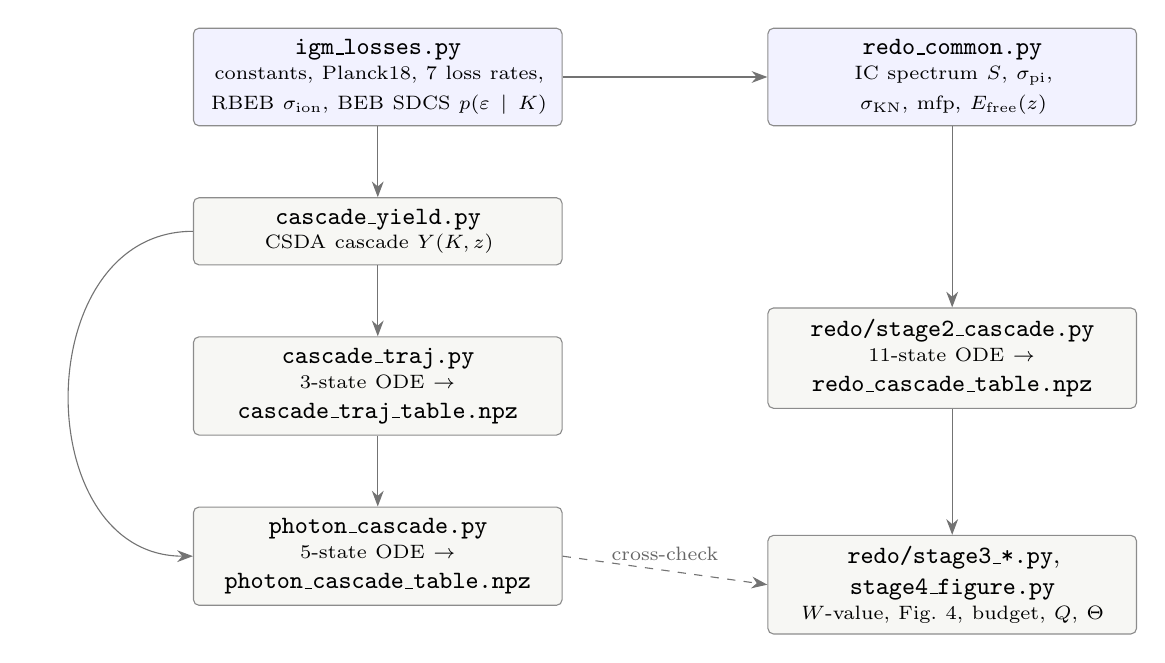
\begin{tikzpicture}[
  node distance=6mm,
  box/.style={draw=black!45, rounded corners=2pt, align=center,
              font=\small, inner sep=4pt, fill=codebg, text width=44mm},
  prim/.style={box, fill=blue!5},
  arr/.style={-{Stealth[length=2mm]}, black!55}]

\node[prim] (igm)  {\file{igm\_losses.py}\\[-2pt]\scriptsize constants, Planck18, 7 loss rates, RBEB $\sion$, BEB SDCS $p(\eps\,\mid\,K)$};
\node[prim, right=26mm of igm] (rc) {\file{redo\_common.py}\\[-2pt]\scriptsize IC spectrum $S$, $\spi$, $\sigma_{\rm KN}$, mfp, $E_{\rm free}(z)$};
\node[box, below=9mm of igm] (cy) {\file{cascade\_yield.py}\\[-2pt]\scriptsize CSDA cascade $Y(K,z)$};
\node[box, below=9mm of cy] (ct) {\file{cascade\_traj.py}\\[-2pt]\scriptsize 3-state ODE $\to$ \file{cascade\_traj\_table.npz}};
\node[box, below=9mm of ct] (pc) {\file{photon\_cascade.py}\\[-2pt]\scriptsize 5-state ODE $\to$ \file{photon\_cascade\_table.npz}};
\node[box, below=9mm of rc, yshift=-14mm] (s2) {\file{redo/stage2\_cascade.py}\\[-2pt]\scriptsize 11-state ODE $\to$ \file{redo\_cascade\_table.npz}};
\node[box, below=16mm of s2] (st3) {\file{redo/stage3\_*.py}, \file{stage4\_figure.py}\\[-2pt]\scriptsize $W$-value, Fig.~4, budget, $Q$, $\Theta$};

\draw[arr] (igm) -- (cy);
\draw[arr] (cy)  -- (ct);
\draw[arr] (ct)  -- (pc);
\draw[arr] (cy.west) to[out=180,in=180,looseness=1.3] (pc.west);
\draw[arr] (igm.east) -- (rc.west);
\draw[arr] (rc) -- (s2);
\draw[arr] (s2) -- (st3);
\draw[arr, dashed] (pc.east) -- node[midway,above,font=\scriptsize,black!60]{cross-check} (st3.west);
\end{tikzpicture}
\end{center}

\noindent
The left column is the production chain used to make the published figure; the
right column is the independent re-derivation.  The two share only
\file{igm\_losses.py}, and only for primitives that are not under test
(constants, cosmology, the seven loss rates, the atomic cross-sections).  The
IC spectrum, its quadrature, the opacity model, the recursion and every
accumulator were written a second time from scratch, with different
quadratures, so that agreement between the two tables is evidence and not a
tautology.

\bigskip
\hrule

%======================================================================
\section{Block-by-block: \file{redo/stage2\_cascade.py}}
%======================================================================

This is the reference implementation: one ODE per grid node, eleven states,
both branches solved together.  Thirteen blocks follow the order of the file.

%----------------------------------------------------------------------
\subsection*{B1 --- Imports and the two names that matter}
%----------------------------------------------------------------------

\begin{lstlisting}
import redo_common as R
import igm_losses as L

EV = R.EV
B  = R.B_H
OUT = Path(__file__).resolve().parent / "redo_cascade_table.npz"
\end{lstlisting}

\code{EV} is the joule value of one electronvolt and \code{B} is
$\BH = 13.6057$~eV.  These two constants are the entire unit convention of the
file: \emph{the ODE state $y_0$ is in joules} (because \code{igm\_losses}
works in SI), while \emph{every energy that indexes a table is in eV}.  Almost
every \code{/ EV} or \code{* EV} in the file is a crossing between those two
conventions, and each one is a place where a bug would be silent.  The two
accumulators fed directly by loss rates, Eqs.~(\ref{eq:dH})--(\ref{eq:dX}),
carry the explicit \code{lr[3] / EV}, \code{lr[4] / EV} for this reason:
$H_q$ and $X_q$ are stored in eV so that $Q = H_q/Y$ comes out in eV per
ionization without further conversion.

%----------------------------------------------------------------------
\subsection*{B2 --- The energy and redshift grids}
%----------------------------------------------------------------------

\begin{lstlisting}
K_LOW  = np.geomspace(0.30, B * 0.995, 9)
K_MAIN = np.concatenate([np.geomspace(B * 1.02, 1e3, 22),
                         np.geomspace(1.3e3, 1e13, 42)])
K_GRID = np.concatenate([K_LOW, K_MAIN])          # 73 nodes
NLOW   = len(K_LOW)
Z_GRID = np.array([5.5, 7.0, 8.5, 10.0, 12.0, 14.0, 17.0, 20.0])
Z_FINAL = 5.5
\end{lstlisting}

Three deliberate features:

\begin{itemize}[leftmargin=1.3em]
\item \code{K\_MAIN} is \emph{identical} to the grid of \file{cascade\_traj.py}.
      That is what makes the comparison between \code{redo\_cascade\_table.npz}
      and \code{cascade\_traj\_table.npz} an element-by-element regression test
      rather than an interpolated comparison.
\item The break at $10^3\to1.3\times10^3$~eV separates the region where the
      yield curve has structure (the $W$ minimum near 100~eV) from the smooth
      power-law region above.  Resolution is spent where the curvature is.
\item \code{K\_LOW}, the nine nodes between 0.30~eV and $0.995\,\BH$, produce
      \emph{no ionizations at all}.  They exist so that a sub-threshold child
      --- a secondary of $\eps<\BH$, or a photoelectron from a photon just above
      the edge --- still has a tabulated $H_q$ and $X_q$ to contribute.  Without
      them each terminating branch of the cascade would silently drop its last
      few eV, and the energy-closure test would fail at the percent level.  This
      was in fact how the closure bug in the static-medium version was found.
\end{itemize}

The redshift nodes are injection redshifts.  Every trajectory ends at
$z=5.5$ or at the thermal floor, whichever comes first.

%----------------------------------------------------------------------
\subsection*{B3 --- The photon-side grids and the two band ceilings}
%----------------------------------------------------------------------

\begin{lstlisting}
_KR = np.geomspace(1.0e5, 1.0e13, 150)          # parent energies that can emit
_EG = np.geomspace(B * (1 + 1e-9), 2.0e3, 160)  # absorbed-photon energies [eV]
EMAX_FIX = np.full(len(Z_GRID), 1.0e3)
EMAX_MFP = np.array([R.e_free(z) for z in Z_GRID])
\end{lstlisting}

\code{\_KR} is the grid on which the photon emission rates are pre-tabulated.
Its floor at $10^5$~eV is a physics statement, not a numerical one: an electron
below $\sim10^5$~eV has $4\gamma^2\langle\eps\rangle < \BH$ and simply cannot
up-scatter a CMB photon above the ionization threshold, so its photon branch is
identically zero and no interpolation is needed there.  \code{\_EG} stops at
2~keV because that is above the largest ceiling in play
($E_{\mathrm{free}}=1820$~eV at $z=20$); the band edge is applied later as a
mask on this grid, so both ceilings are served by one tabulation.

\code{EMAX\_MFP} calls \code{redo\_common.e\_free(z)}, which solves
$\lambda_\gamma(E,z) = c/H(z)$ by bisection.  Note that the mean free path
combines photoionization \emph{and} Klein--Nishina scattering,
\[
  \lambda_\gamma^{-1} = \nHI\,\spi(\Eg) + (1+x_e)\,\nHI\,\sigma_{\mathrm{KN}}(\Eg),
\]
so \code{e\_free} is the energy at which a photon stops interacting at all,
not the energy at which it stops photoionizing.  That distinction is what
makes the one-absorption rule optimistic by 5--13\,\% for this ceiling
(Sect.~2.3 of the counting note): near the edge, a third of the interactions
are Compton scatters that do not ionize.

%----------------------------------------------------------------------
\subsection*{B4 --- \code{photon\_spectra()}: the emission cube}
%----------------------------------------------------------------------

\begin{lstlisting}
def photon_spectra():
    """S[z, K, Eg] = dN/(dt dE_gamma) [s^-1 eV^-1]; computed once."""
    S = np.zeros((len(Z_GRID), len(_KR), len(_EG)))
    for iz, z in enumerate(Z_GRID):
        for ik, K in enumerate(_KR):
            S[iz, ik] = R.ic_dnde(K, z, _EG)
    return S
\end{lstlisting}

$8\times150\times160 = 192{,}000$ numbers, each a Klein--Nishina kernel
integrated over the Planck spectrum, evaluated once at the top of the run.
This is the single most important optimisation in the file: the same spectrum
would otherwise be recomputed inside every right-hand-side evaluation, tens of
millions of times.  Because $S$ is linear in the seed photon density and the
$z$-dependence of the CMB is a pure scaling, nothing in the cube depends on the
cascade, so it can be built before the march starts.

%----------------------------------------------------------------------
\subsection*{B5 --- \code{band\_moments()}: turning a spectrum into event rates}
%----------------------------------------------------------------------

\begin{lstlisting}
def band_moments(S, child_Y, child_H):
    """(R0, Reff, Rheat) for the fixed and the mfp ceiling."""
    out = {}
    for tag, emax in (("f", EMAX_FIX), ("m", EMAX_MFP)):
        ...
        for iz, z in enumerate(Z_GRID):
            m  = _EG <= emax[iz]
            Eg = _EG[m]
            Ke = np.maximum(Eg - B, 0.0)
            yv = child_Y(z, Ke)
            hv = child_H(z, Ke)
            s  = S[iz][:, m]
            R0[iz] = np.trapz(s, Eg, axis=1)
            Re[iz] = np.trapz(s * (1.0 + yv[None, :]), Eg, axis=1)
            Rh[iz] = np.trapz(s * hv[None, :], Eg, axis=1)
        out[tag] = (R0, Re, Rh)
    return out
\end{lstlisting}

This block \emph{is} the photon counting rule, Eq.~(\ref{eq:moments}).  Four
things are worth stating explicitly because they are invisible in the code:

\begin{enumerate}[leftmargin=1.6em]
\item \textbf{The band is a mask, not a weight.}  \code{m = \_EG <= emax[iz]}
      is a hard cut.  Inside the band the absorption probability is unity;
      outside it is zero.  $\spi$ never appears in this function --- it entered
      only through \code{e\_free}, i.e.\ only in \emph{locating} the ceiling.
\item \textbf{The \code{1.0 +} in \code{Re} is the photoionization itself.}
      \code{yv} is what the photoelectron goes on to do; the leading 1 is the
      bound electron that the photon removed.  Dropping it would lose roughly
      a quarter of $Y_\gamma$ at the plateau.
\item \textbf{\code{Ke = Eg - B}} implements the kinematics of photoabsorption:
      the photoelectron carries the photon energy minus the binding energy,
      and \code{np.maximum(...,0)} guards the first grid point, which sits
      $10^{-9}$ of a threshold above $\BH$.
\item \textbf{\code{R0} deliberately omits the \code{1.0 +}.}  $N_\gamma$ is a
      photon count, $Y_\gamma$ an ionization count; the ratio
      $Y_\gamma/N_\gamma$ is the ``ionizations per productive photon'' number
      ($3.60$), so the two must be accumulated on the same footing.  They are
      here; they are not in the production code (Sect.~\ref{sec:prod}).
\end{enumerate}

The trapezoid integrals run along the last axis for all 150 parent energies at
once, which is why the cube is stored $[z,K,\Eg]$ rather than $[\Eg,K,z]$.

%----------------------------------------------------------------------
\subsection*{B6 --- \code{\_log\_interp\_stack()}: six rates, one lookup}
%----------------------------------------------------------------------

\begin{lstlisting}
def _log_interp_stack(tabs):
    """One vector-valued interpolator for all six photon rates (log space)."""
    v = np.log(np.clip(np.stack(tabs, axis=-1), 1e-300, None))
    return RegularGridInterpolator((Z_GRID, np.log(_KR)), v,
                                   bounds_error=False, fill_value=None)
\end{lstlisting}

The six tables are $(R_0,R_{\mathrm{eff}},R_h)$ for each of the two ceilings.
Two design choices:

\begin{itemize}[leftmargin=1.3em]
\item \textbf{Logarithms in all three directions.}  $R_0$ spans some thirty
      decades across \code{\_KR}, and near the emission threshold it falls off
      faster than any polynomial.  Linear interpolation of the raw values would
      be catastrophically wrong there; linear interpolation of $\ln R$ against
      $\ln K$ is accurate because the tables are locally power laws.  The
      \code{clip(1e-300)} keeps $\ln 0$ out of the table.
\item \textbf{One vector-valued interpolator instead of six scalar ones.}
      \code{RegularGridInterpolator} with a trailing value axis returns all six
      numbers per call.  The right-hand side is evaluated of order $10^7$ times
      over a full run, so collapsing six Python-level calls into one was worth
      roughly a factor two in wall time.  The same trick is applied to the ten
      shower averages in B8; together they took the run from an estimated
      $\sim$50~min to the 1313~s it actually took.
\end{itemize}

\code{fill\_value=None} means linear extrapolation outside the box rather than
NaN; in practice the caller always clips first, so this only guards rounding at
the edges.

%----------------------------------------------------------------------
\subsection*{B7 --- \code{child\_interp()}: what a photoelectron will do}
%----------------------------------------------------------------------

\begin{lstlisting}
def child_interp(vals, n_done):
    if n_done < 2:
        return lambda z, K: np.zeros_like(np.atleast_1d(K), dtype=float)
    Kk = K_GRID[:n_done]
    f = RegularGridInterpolator((Z_GRID, np.log(Kk)), vals[:, :n_done], ...)
    def g(z, K):
        K  = np.atleast_1d(np.asarray(K, float))
        lk = np.clip(np.log(np.clip(K, Kk[0], None)), np.log(Kk[0]), np.log(Kk[-1]))
        zz = np.full(lk.size, np.clip(z, Z_GRID[0], Z_GRID[-1]))
        return np.maximum(f(np.column_stack([zz, lk])), 0.0)
    return g
\end{lstlisting}

A closure over the part of the table that is already known.  \code{n\_done} is
the number of completed rows of the upward march, so \code{child\_interp}
physically encodes ``a child can only be looked up at an energy the march has
already passed''.  Three defensive details:

\begin{itemize}[leftmargin=1.3em]
\item the double \code{clip} pins $K$ into $[K_{\mathrm{grid}}[0],
      K_{\mathrm{grid}}[n_{\mathrm{done}}-1]]$ before the logarithm, so a
      photoelectron of $10^{-3}$~eV is treated as one of $0.30$~eV.  For $Y$
      that is exact (both give zero); for $H_q$ it slightly over-credits the
      softest photoelectrons, by at most $0.3$~eV each;
\item \code{np.maximum(\ldots,0)} kills the small negative excursions that
      linear interpolation of a convex table can produce near the threshold
      kink at $\BH$;
\item the \code{n\_done < 2} branch returns a zero function, so the very first
      grid node --- which has no children below it --- is handled without a
      special case in the caller.
\end{itemize}

%----------------------------------------------------------------------
\subsection*{B8 --- \code{fill\_shower\_row()}: the recursion, and why it is one-pass}
%----------------------------------------------------------------------

\begin{lstlisting}
def fill_shower_row(cache, res, ik, pdfs):
    """<Q(eps,z)> for a parent at K_GRID[ik], for all ten accumulators.

    A secondary always has eps < K_GRID[ik], so the row is final once row ik of
    every accumulator is known: it never has to be recomputed.
    """
    eps, pdf = pdfs[ik]
    if eps is None:
        return
    Kk = K_GRID[:ik + 1]
    for iz in range(len(Z_GRID)):
        for j, k in enumerate(KEYS):
            cache[iz, ik, j] = np.trapz(
                pdf * np.interp(eps, Kk, res[k][iz, :ik + 1], left=0.0), eps)
\end{lstlisting}

This is the numerical heart of the whole calculation.  It evaluates
\[
  \bigl\langle Q(\eps,z)\bigr\rangle \;=\;
  \int_0^{(K-\BH)/2} p(\eps\,|\,K)\; Q(\eps,z)\, d\eps
\]
for all ten accumulators $Q \in \{N_1, Y, H_q, X_q, N_\gamma^{f}, Y_\gamma^{f},
H_\gamma^{f}, N_\gamma^{m}, Y_\gamma^{m}, H_\gamma^{m}\}$ at once.

The docstring states the causality argument that makes the scheme exact in a
single sweep.  By the BEB convention the ``secondary'' is the \emph{slower} of
the two outgoing electrons, so $\eps \le (K-\BH)/2 < K$ strictly.  A parent at
$K_{\mathrm{grid}}[ik]$ therefore only ever interpolates $Q$ at energies that
the march has already resolved, and---this is the part that matters for
performance---row \code{ik} of the cache can never change afterwards.  It is
written once and never revisited.  A scheme that did not have this property
would need outer iterations to convergence, at $73\times 8$ stiff ODEs per
iteration.

\code{left=0.0} in the \code{np.interp} is the statement that a secondary below
the lowest grid node contributes nothing; combined with \code{K\_LOW} reaching
down to 0.30~eV, the truncation error this introduces is under a tenth of an eV
per branch.

Note that $j=0$, the average $\langle N_1\rangle$, is computed but never used:
$N_1$ is by definition the primary's own count and carries no shower term.  It
is kept in the loop only so that the ten accumulators can share one array
layout and one interpolator.

%----------------------------------------------------------------------
\subsection*{B9 --- \code{shower\_interp\_all()}}
%----------------------------------------------------------------------

\begin{lstlisting}
def shower_interp_all(cache, n_done):
    if n_done < 2:
        return None
    return RegularGridInterpolator(
        (Z_GRID, np.log(K_GRID[:n_done])), cache[:, :n_done, :], ...)
\end{lstlisting}

The counterpart of B6 for the shower side: one vector-valued interpolator
returning all ten $\langle Q\rangle$ per call.  Unlike the photon rates this
table is \emph{not} interpolated in logarithm of the value, because several of
the accumulators are legitimately zero over a wide range (any $\langle
Y_\gamma\rangle$ below $10^5$~eV, all of them below $\BH$) and $\ln 0$ has no
useful linear behaviour.  The values themselves are smooth and $O(1)$ to
$O(10^6)$, so linear interpolation against $\ln K$ is adequate; the
\code{np.maximum(\ldots,0)} at the call site cleans up the undershoot.

%----------------------------------------------------------------------
\subsection*{B10 --- \code{run()}: set-up}
%----------------------------------------------------------------------

\begin{lstlisting}
res = {k: np.zeros((nZ, nK)) for k in KEYS}
sec_cache = np.zeros((nZ, nK, len(KEYS)))

S = photon_spectra()

pdfs = []
for K in K_GRID:
    e, p = R.secondary_pdf(K) if K > B else (None, None)
    if e is not None:
        m = e > 0
        pdfs.append((e[m], p[m]))
    else:
        pdfs.append((None, None))

ms = None       # vector interpolator of <Q(eps,z)>
rates = None    # vector interpolator of the photon rates
\end{lstlisting}

\code{res} holds the answer; \code{sec\_cache} holds the shower averages;
\code{pdfs} pre-computes the 73 BEB secondary spectra so they are never rebuilt
inside the ODE.  \code{ms} and \code{rates} start as \code{None}, which is the
signal that ``nothing is known yet'' --- the first grid node runs with both
recursion terms identically zero, which is correct because a $0.30$~eV electron
has neither a shower nor a photon branch.

%----------------------------------------------------------------------
\subsection*{B11 --- The right-hand side}
%----------------------------------------------------------------------

\begin{lstlisting}
def rhs(t, y):
    KJ = max(float(y[0]), 0.0)
    if KJ <= 0.0:
        return [0.0] * 11
    z    = float(L.z_interp(t))
    KeV  = KJ / EV
    lr   = np.asarray(L.loss_rates(z, KJ, float(L.H_interp(t)), L.toggles()), float).ravel()
    tot  = float(lr.sum())
    _, _, _, v = L.kinematics(KJ)
    rc   = L.n_HI(z) * float(v) * float(R.sigma_ion(KeV))

    zc = float(np.clip(z, Z_GRID[0], Z_GRID[-1]))
    if ms is not None and ik:
        lk  = float(np.clip(np.log(max(KeV, K_GRID[0])),
                            np.log(K_GRID[0]), np.log(K_GRID[ik - 1])))
        sec = np.maximum(np.ravel(ms(((zc, lk),))), 0.0)
    else:
        sec = ZERO_S

    if rates is not None and KeV >= _KR[0]:
        lk = float(np.clip(np.log(KeV), np.log(_KR[0]), np.log(_KR[-1])))
        ph = np.exp(np.ravel(rates(((zc, lk),))))
    else:
        ph = ZERO_R

    return [
        -tot,                          # dK/dt
        rc,                            # dN1/dt
        rc * (1.0 + sec[1]),           # dY/dt
        lr[3] / EV + rc * sec[2],      # dHq/dt   (lr[3] = Coulomb)
        lr[4] / EV + rc * sec[3],      # dXq/dt   (lr[4] = excitation)
        ph[0] + rc * sec[4],           # dNg_fixed/dt
        ph[1] + rc * sec[5],           # dYph_fixed/dt
        ph[2] + rc * sec[6],           # dHph_fixed/dt
        ph[3] + rc * sec[7],           # ... same three, mfp ceiling
        ph[4] + rc * sec[8],
        ph[5] + rc * sec[9],
    ]
\end{lstlisting}

Line by line:

\begin{description}[leftmargin=0pt,style=unboxed,itemsep=3pt]
\item[\code{z = L.z\_interp(t)}] The integration variable is cosmic time, not
      redshift.  \code{z\_interp} and \code{H\_interp} are pre-built splines of
      the Planck18 background, so no cosmology call happens inside the ODE.
\item[\code{lr = L.loss\_rates(...)}] Returns the seven channels in the fixed
      order (adiabatic, synchrotron, IC, Coulomb, excitation, ionization,
      bremsstrahlung).  \code{tot} drives $K$; \code{lr[3]} and \code{lr[4]}
      are \emph{additionally} tapped as source terms for the heat and
      excitation accumulators.  The other five channels are not accumulated
      here --- they are reconstructed afterwards as the escaping remainder,
      which is what makes the closure test independent.
\item[\code{rc = n\_HI * v * sigma\_ion}] Eq.~(\ref{eq:rc}).  This single
      quantity drives \emph{four} different accumulators: the primary count,
      the shower count, and the shower's contribution to the heat and to both
      photon branches.  Every appearance of \code{rc * sec[j]} says ``at this
      instant the primary makes $r_c\,dt$ secondaries, and each of them will
      eventually contribute $\langle Q\rangle$''.
\item[the \code{clip} to \code{K\_GRID[ik-1]}] The parent at node \code{ik}
      may only consult shower data strictly below itself.  Because the primary
      starts exactly at $K_{\mathrm{grid}}[ik]$ and cools, this clip is active
      only for the first instants of the trajectory, and the error it makes
      there is bounded by one grid spacing in $\ln K$.
\item[\code{ph = np.exp(rates(...))}] Undoes the logarithm of B6.  The guard
      \code{KeV >= \_KR[0]} enforces the physical statement of B3: below
      $10^5$~eV the photon branch is exactly zero, not merely small.
\item[the return list] is precisely
      Eqs.~(\ref{eq:dK})--(\ref{eq:dHg}), with the last three repeated for the
      second ceiling.  Note \code{dN1/dt = rc} alone: the primary's own count
      never receives a shower term, which is what makes the multiplicity
      $Y/N_1$ (1.00 at 40~eV rising to $\sim$2.5 at the top of the grid) a
      meaningful diagnostic.
\end{description}

%----------------------------------------------------------------------
\subsection*{B12 --- The stopping condition and the integrator}
%----------------------------------------------------------------------

\begin{lstlisting}
def ev(t, y):
    return y[0] - float(L.thermal_floor(L.z_interp(t)))
ev.terminal, ev.direction = True, -1

sol = solve_ivp(rhs, (t_i, t_f), [K0 * EV] + [0.0] * 10,
                events=ev, method="Radau", rtol=1e-6, atol=1e-25)
for j, k in enumerate(KEYS):
    res[k][iz, ik] = sol.y[j + 1, -1]
\end{lstlisting}

Three points:

\begin{itemize}[leftmargin=1.3em]
\item \textbf{The terminal event} stops the integration when the electron
      reaches $1.5\,k_B T_{\mathrm{CMB}}(z)$, i.e.\ when it has thermalised.
      Without it the solver would chase an exponentially decaying $K$ to
      $t_f$ at enormous cost, and the adiabatic term would keep producing
      meaningless small numbers.  \code{direction=-1} makes it fire only on the
      downward crossing.
\item \textbf{\code{method="Radau"}} is not optional.  The system is violently
      stiff: at $10^{12}$~eV the IC time-scale is many orders of magnitude
      shorter than the Hubble time that sets the integration span, and the
      Coulomb term stiffens again at the bottom.  An explicit method either
      fails or takes $10^{6}$ steps.
\item \textbf{\code{atol=1e-25}} looks extreme but is set by the units: $y_0$
      is in joules, so a $1$~eV electron is $y_0\sim10^{-19}$.  An absolute
      tolerance of $10^{-25}$~J is $\sim10^{-6}$~eV, which is the right scale.
      The accumulators, being $O(1)$ to $O(10^6)$, are controlled by
      \code{rtol} alone.
\end{itemize}

Only the final value of each accumulator is kept: \code{sol.y[j+1, -1]}.  The
trajectory itself is discarded, which is why the file is fast to load and small
on disk.

%----------------------------------------------------------------------
\subsection*{B13 --- Closing the row, and the 4~keV freeze}
%----------------------------------------------------------------------

\begin{lstlisting}
fill_shower_row(sec_cache, res, ik, pdfs)
ms = shower_interp_all(sec_cache, ik + 1)

# The photon branch only ever needs child yields below ~2 keV, so the
# band moments stop changing once the marching has passed that energy.
if K_GRID[ik] < 4.0e3 or rates is None:
    cY  = child_interp(res["Y"],  ik + 1)
    cH  = child_interp(res["Hq"], ik + 1)
    mom = band_moments(S, cY, cH)
    rates = _log_interp_stack([mom["f"][0], mom["f"][1], mom["f"][2],
                               mom["m"][0], mom["m"][1], mom["m"][2]])
\end{lstlisting}

The first two lines advance the recursion by exactly one node: the row just
computed is folded into the shower cache and a fresh interpolator is built.
Both are $O(n_K n_Z)$, negligible against the eight stiff ODEs that preceded
them.

The \code{if} is a genuine physics optimisation and deserves the comment it
has.  \code{band\_moments} is expensive ($2\times8\times150\times160$ trapezoid
evaluations) and would otherwise be rebuilt 73 times.  But it only ever queries
the child tables at $K_e = \Eg - \BH \le 2\ \mathrm{keV} - \BH$.  Once the
upward march has passed 4~keV, every child energy the photon branch can ask for
is already final, so the moments are frozen.  This is safe precisely because of
the same causality property as B8, and it is worth roughly a third of the total
run time.

Finally, the whole \code{res} dictionary is written to
\file{redo\_cascade\_table.npz} every fourth node as well as at the end, so a
run that dies at hour two is not a total loss; \code{done=ik+1} records how far
it got.

%----------------------------------------------------------------------
\subsection{The cost, and why it is arranged this way}
%----------------------------------------------------------------------

\begin{center}
\begin{tabular}{lr}
\toprule
Stiff ODE integrations (73 energies $\times$ 8 redshifts) & 584 \\
States per integration                                    & 11 \\
IC spectra tabulated once                                 & $1.9\times10^{5}$ \\
BEB secondary spectra tabulated once                      & 73 \\
\code{band\_moments} rebuilds (with the 4~keV freeze)      & 32 of 73 \\
Wall time, single core                                    & 1312.8~s \\
\bottomrule
\end{tabular}
\end{center}

The structure is dictated entirely by the recursion.  The physics would allow
each $(K_0,z_i)$ to be solved independently \emph{if} $Y$ at lower energies were
already known; it is not, so the march must be serial in $K$.  It can be, and
is, parallel in $z$ --- the eight redshifts at fixed $K$ are independent --- but
at 584 integrations the serial version was fast enough not to bother.

\bigskip
\hrule

%======================================================================
\section{The upstream blocks the cascade rests on}
%======================================================================

The cascade solver is thin; almost all of the physics enters through four
primitives.  Each is worth one block.

%----------------------------------------------------------------------
\subsection*{U1 --- \code{igm\_losses.coll\_ionisation\_cross\_section}: $\sion(K)$}
%----------------------------------------------------------------------

The relativistic binary-encounter-Bethe cross-section (Kim, Santos \& Parente
2000).  For H(1s) it is written in terms of $t = K/\BH$ and the reduced
kinematic variables $\beta_t^2,\beta_u^2,\beta_b^2$, with the dipole
oscillator-strength distribution entering through the fitted coefficients

\begin{lstlisting}
_DIPOLE_FIT = np.array([-0.0224728, 1.177455, -0.4626461, 0.08906479])
\end{lstlisting}

It returns exactly $0$ for $K \le \BH$.  That hard zero is what terminates every
branch of the cascade tree: a secondary below threshold simply stops
contributing, with no cut-off having to be imposed by hand.

In \file{redo\_common} the function is re-exported with a vectorising wrapper,
because the original takes scalars only:

\begin{lstlisting}
def sigma_ion(K_eV):
    K_eV = np.atleast_1d(np.asarray(K_eV, float))
    out = np.array([L.coll_ionisation_cross_section(k * EV) if k > B_H else 0.0
                    for k in K_eV])
    return out if out.size > 1 else float(out[0])
\end{lstlisting}

%----------------------------------------------------------------------
\subsection*{U2 --- \code{beb\_sdcs} / \code{secondary\_pdf}: $p(\eps\,|\,K)$}
%----------------------------------------------------------------------

\begin{lstlisting}
def beb_sdcs(w, t):
    """dsigma/dw [m^2] for a primary at t = K/B and a secondary at w = eps/B."""
    return (_BEB_S / (t + _BEB_U + 1.0)) * (
        (_BEB_NI - 2.0) / (t + 1.0) * (1.0 / (1.0 + w) + 1.0 / (t - w))
        + (2.0 - _BEB_NI) * (1.0 / (1.0 + w) ** 2 + 1.0 / (t - w) ** 2)
        + np.log(t) / (1.0 + w) * _beb_dfdw(w))

def secondary_pdf(K_eV, n=300):
    t = float(K_eV) / THRESHOLD_EV_ION
    w_max = (t - 1.0) / 2.0                       # <- the causality bound
    if w_max <= 0.0:
        return None, None
    w = np.geomspace(max(1e-6, 1e-6 * w_max), w_max, n)
    d = np.maximum(beb_sdcs(w, t), 0.0)
    norm = np.trapz(d, w)
    return w * THRESHOLD_EV_ION, d / norm / THRESHOLD_EV_ION
\end{lstlisting}

Two structural facts follow from these ten lines and are used everywhere:

\begin{enumerate}[leftmargin=1.6em]
\item \code{w\_max = (t-1)/2}, i.e.\ $\eps_{\max}=(K-\BH)/2$.  This is the whole
      justification for the one-pass upward march.  It is not an approximation:
      it is the BEB convention that the ejected electron is the slower of the
      two.
\item The cross-section is built from \emph{the same} \code{\_DIPOLE\_FIT}
      coefficients as the total cross-section of U1.  Integrating the
      differential form reproduces the total to $0.01\,\%$ below 300~eV and
      $2.6\,\%$ at 10~keV, so the rate at which events occur and the spectrum
      of what they produce are the same physics rather than two unrelated fits.
      This matters: a mismatch here would break energy conservation in a way
      the closure test would catch but not diagnose.
\end{enumerate}

Note that the pdf is normalised to unit \emph{probability}, not to
$\sion$; the cross-section magnitude enters separately through $r_c$.

%----------------------------------------------------------------------
\subsection*{U3 --- \code{igm\_losses.loss\_rates}: the seven channels}
%----------------------------------------------------------------------

Returns a stacked array of seven positive rates in J~s$^{-1}$, in a fixed
order that the cascade code depends on by index:

\begin{center}
\begin{tabular}{clll}
\toprule
index & channel & used for $dK/dt$ & tapped separately \\
\midrule
0 & adiabatic expansion       & yes & --- \\
1 & synchrotron               & yes & --- \\
2 & inverse Compton (KN)      & yes & --- (the photon branch uses $S$, not $L_{\rm IC}$) \\
3 & Coulomb (Gould 1972)      & yes & $\to dH_q/dt$ \\
4 & collisional excitation    & yes & $\to dX_q/dt$ \\
5 & collisional ionization    & yes & --- (the count uses $\sion$, not $L_{\rm ion}$) \\
6 & bremsstrahlung            & yes & --- \\
\bottomrule
\end{tabular}
\end{center}

Rows 2 and 5 are the two places where the code deliberately does \emph{not}
reuse the loss rate for counting:

\begin{itemize}[leftmargin=1.3em]
\item \textbf{Ionization.}  $L_{\mathrm{ion}} = \nHI v\, \sion (\BH +
      \langle\eps\rangle)$ is an \emph{energy} loss; the event rate is
      $\nHI v\, \sion$.  Dividing one by the other would give the right number
      only if every secondary carried exactly $\langle\eps\rangle$.  Keeping
      them separate is what makes the no-double-counting argument work: the
      parent is charged $\BH + \langle\eps\rangle$ per event, the child spends
      exactly $\eps$, and the event is counted once.
\item \textbf{Inverse Compton.}  $L_{\mathrm{IC}}$ says how much energy is
      radiated, not how many photons land in the band.  Hence the differential
      spectrum of U4.  As a consistency check, the energy integral of that
      spectrum reproduces $L_{\mathrm{IC}}$ to $0.14\,\%$ in the relativistic
      regime, of which $0.115\,\%$ is the rounded constant
      $U_{\mathrm{CMB},0}=4.17\times10^{-14}$~J~m$^{-3}$ versus the exact
      $aT^4$, and the remainder is the exact factor
      $\gamma^2/(\gamma^2-1)=1/\beta^2$ between emitted and net power.
\end{itemize}

%----------------------------------------------------------------------
\subsection*{U4 --- \code{redo\_common.ic\_dnde}: the IC photon spectrum}
%----------------------------------------------------------------------

\begin{lstlisting}
_XN = 801
_LX = np.linspace(np.log(1.0e-5), np.log(80.0), _XN)
_XG = np.exp(_LX)
_SIMP = np.ones(_XN); _SIMP[1:-1:2] = 4.0; _SIMP[2:-1:2] = 2.0
_SIMP *= (_LX[1] - _LX[0]) / 3.0
_W_NUMBER = _SIMP * _XG * _XG / np.expm1(_XG)     # extra x from dx = x dlnx

def ic_dnde(K_eV, z, Eg_eV):
    gamma = 1.0 + float(K_eV) / E0_EV
    kT  = KT0 * (1.0 + float(z))
    eps = _XG * kT
    Gam = 4.0 * gamma * eps / L.E0
    EgJ = Eg[:, None] * EV
    den = Gam[None, :] * (gamma * L.E0 - EgJ)
    q   = np.divide(EgJ, den, out=np.full_like(den, np.inf), where=den > 0.0)
    ok  = (q >= 1.0 / (4.0 * gamma**2)) & (q <= 1.0)
    qs  = np.clip(q, 1.0e-300, 1.0)
    Gq  = Gam[None, :] * qs
    G   = (2.0*qs*np.log(qs) + (1.0 + 2.0*qs)*(1.0 - qs)
           + 0.5*Gq**2*(1.0 - qs)/(1.0 + Gq))
    G   = np.where(ok, np.maximum(G, 0.0), 0.0)
    pref = 3.0 * L.THOMSON_CROSS_SECTION_MKS * L.C_LIGHT / (4.0 * gamma**2)
    return pref * _planck_prefactor(kT) * (G @ _W_NUMBER) * EV
\end{lstlisting}

This is Blumenthal \& Gould (1970), Eq.~(2.48), integrated over a Planck seed
spectrum:
\[
  \frac{dN_\gamma}{dt\,d\Eg} =
  \frac{3\sigma_T c}{4\gamma^2}\int \frac{n(\eps)}{\eps}\,G(q,\Gamma)\,d\eps,
  \qquad
  q = \frac{\Eg}{\Gamma(\gamma m c^2 - \Eg)},\quad
  \Gamma = \frac{4\gamma\eps}{m c^2}.
\]

Implementation notes:

\begin{itemize}[leftmargin=1.3em]
\item The seed integral is done as a composite Simpson rule on a logarithmic
      grid in $x=\eps/k_BT$, over $10^{-5}<x<80$, deliberately \emph{different}
      from the 128-node Gauss--Legendre rule used by
      \file{photon\_cascade.py}.  The two share no nodes and no weights, so the
      agreement of the resulting yields is a real check on the quadrature.
\item The mask \code{ok} enforces the two kinematic limits: $q\le 1$ is the
      full-energy-transfer bound $\Eg<\gamma mc^2$, and $q\ge 1/(4\gamma^2)$ is
      the floor at which the photon leaves with the energy it came in with.
      Outside that range the kernel is set to zero rather than allowed to go
      negative, which it otherwise does.
\item The final $\times$\code{EV} converts from per-joule to per-eV, matching
      the eV grid \code{\_EG} that \code{band\_moments} integrates over.  This
      is the one unit crossing on the photon side, and it is the reason the
      band moments come out in s$^{-1}$ rather than s$^{-1}$J$^{-1}$.
\item The matrix product \code{G @ \_W\_NUMBER} does all 160 photon energies
      against all 801 seed nodes in one call.  Given how many times the cube is
      built, this vectorisation is what keeps \code{photon\_spectra()} to a few
      seconds.
\end{itemize}

%----------------------------------------------------------------------
\subsection*{U5 --- The opacity block: \code{sigma\_pi}, \code{sigma\_kn}, \code{e\_free}}
%----------------------------------------------------------------------

\begin{lstlisting}
SIGMA_PI_THRESHOLD = 6.30e-18 * 1.0e-4          # m^2, H(1s) at 13.6 eV

def sigma_pi(E_eV):                              # Karzas & Latter (1961)
    x = E_eV / B_H
    e = np.sqrt(x - 1.0)
    return (SIGMA_PI_THRESHOLD * x**-4 * np.exp(4.0 - 4.0*np.arctan(e)/e)
            / (1.0 - np.exp(-2.0*np.pi/e)))

def photon_mfp(E_eV, z):
    nH = L.n_HI(z)
    return 1.0 / (nH*sigma_pi(E_eV) + (1.0 + L.ION_FRACTION)*nH*sigma_kn(E_eV))

def e_free(z):
    f = lambda lg: photon_mfp(10.0**lg, z) / hubble_length(z) - 1.0
    return 10.0 ** brentq(f, np.log10(20.0), 5.0, xtol=1e-10)
\end{lstlisting}

$\spi \propto E^{-3}$ asymptotically, so the IGM becomes transparent very
quickly above threshold; \code{e\_free} finds where it becomes transparent on
the scale of the horizon, giving 1820~eV at $z=20$ down to 983~eV at $z=5.5$.

The essential remark, repeated from B5: \emph{this is the only place $\spi$
enters the ionization count}.  Inside the band the code does not use it at all.
The accuracy of that shortcut was measured separately (\file{stage3\_opacity.py})
by forming the photon-weighted probability that a band photon is absorbed
\emph{as a photoionization} within one Hubble length:
$0.99$ for the fixed 1~keV band, $0.87$--$0.95$ for the horizon ceiling.

\bigskip
\hrule

%======================================================================
\section{The production pair, and where it differs}
\label{sec:prod}
%======================================================================

The published figure was made by two files rather than one.

\subsection*{P1 --- \file{cascade\_traj.py}: the electron branch alone}

Three states, $(K, N_1, Y)$, and a single scalar shower average:

\begin{lstlisting}
def rhs(t, y):
    ...
    rate = L.n_HI(z) * float(v) * float(sigma_ion(K / EV))
    sec  = _mean_shower(K / EV, z, Y, ik, ms) if ik else 0.0
    return [-tot, rate, rate * (1.0 + sec)]
\end{lstlisting}

Structurally identical to Eqs.~(\ref{eq:dK})--(\ref{eq:dY}); the recursion is
closed by the same upward march, with \code{\_build\_ms\_interp} playing the
role of B8 for the single quantity $Y$.  Output:
\file{cascade\_traj\_table.npz}.

\subsection*{P2 --- \file{cascade\_yield.py}: the CSDA child table}

\begin{lstlisting}
def solve_Y(z, Kg=K_NODES):
    sig, Lam_tot = stopping(z, Kg)
    r = np.where(Lam_tot > 0, sig / Lam_tot, 0.0)     # ionizations per eV lost
    Y = np.zeros_like(Kg)
    for i in range(1, len(Kg)):
        dK    = Kg[i] - Kg[i - 1]
        e, p  = secondary_pdf(0.5 * (Kg[i] + Kg[i - 1]))
        Yi    = np.interp(e, Kg[:i], Y[:i], left=0.0)
        Yi[e < B] = 0.0
        Ys    = float(np.trapz(p * Yi, e))
        Y[i]  = Y[i - 1] + dK * 0.5 * (r[i] + r[i - 1]) * (1.0 + Ys)
\end{lstlisting}

The same cascade equation solved without any ODE, in the continuous
slowing-down approximation:
\[
  Y(K,z) = \int^{K} \frac{\sion(K')}{\Lambda_{\rm tot}(K')}
           \bigl[1 + \langle Y(\eps,z)\rangle_{p(\eps|K')}\bigr]\,dK' .
\]
It is valid for children only, because an electron below $\sim10^5$~eV
thermalises in $\Delta z \ll 1$ and the medium does not change underneath it.
\code{build\_table()} caches it on \code{K\_NODES} $\in[10.2, 10^6]$~eV.  In the
redo this file is not used at all: children are looked up in the same
trajectory-solved table as parents, which removes the CSDA approximation from
the child side entirely.  The two agree to about 1\,\% in $Q$, which is a
useful independent measure of how good CSDA is here.

\subsection*{P3 --- \file{photon\_cascade.py}: the photon branch bolted on}

Five states, $(K, N_\gamma^f, N_\gamma^m, Y_\gamma^f, Y_\gamma^m)$, with
$Y_{\mathrm e}$ \emph{not} recomputed:

\begin{lstlisting}
direct = np.load(... "cascade_traj_table.npz")
if not (np.allclose(direct["K"], K_GRID) and np.allclose(direct["z"], Z_GRID)):
    raise RuntimeError("cascade_traj_table.npz is not on the expected grid")
N1 = direct["N1"].copy()
Ye = direct["Y"].copy()
...
return [-tot, r0f, r0m, rc * sf + reff, rc * sm + remf]
\end{lstlisting}

Reusing the electron table avoids several hundred redundant stiff
integrations, and the explicit grid assertion turns that reuse into a
regression check.

\subsection*{P4 --- The four differences that matter}

\begin{center}
\begin{tabular}{p{4.6cm}p{4.6cm}p{5.6cm}}
\toprule
& production pair & \file{redo/stage2\_cascade.py} \\
\midrule
Photoelectron yield $Y_{\rm e}(\Eg-\BH)$
  & from the CSDA table of \file{cascade\_yield.py}
  & from the trajectory table itself \\[3pt]
Seed-photon quadrature
  & 128-node Gauss--Legendre in $x$, 180-point $\Eg$ grid
  & 801-point Simpson in $\ln x$, 160-point $\Eg$ grid \\[3pt]
Shower term in the photon \emph{count}
  & \code{r0f} only: $N_\gamma$ omits $r_c\langle N_\gamma\rangle$ while
    $Y_\gamma$ includes $r_c\langle Y_\gamma\rangle$
  & \code{ph[0] + rc*sec[4]}: both include it \\[3pt]
Heat / excitation accumulators
  & absent
  & \code{Hq}, \code{Xq}, \code{Hpf}, \code{Hpm} carried, enabling the closure
    test and $Q=H_q/Y$ \\
\bottomrule
\end{tabular}
\end{center}

The third row is the one to be aware of when quoting numbers: the published
``3.6 ionizations per productive photon'' is a ratio whose numerator and
denominator use different conventions.  With both accumulators consistent the
ratio is still $3.60$, so nothing downstream changes, but the two quantities as
tabulated are not on the same footing.

\bigskip
\hrule

%======================================================================
\section{How the implementation is checked}
%======================================================================

\begin{description}[leftmargin=0pt,style=unboxed,itemsep=4pt]
\item[Energy closure.]  $\BH Y + H_q + X_q + E_{\rm esc} = K_{\rm ini}$ holds
      to $0.4\,\%$ along the trajectory and to $0.03\,\%$ in the static
      version, where there is no ODE tolerance.  $E_{\rm esc}$ is reconstructed
      as the remainder, so this test genuinely closes the loop rather than
      restating it.
\item[Table-vs-table.]  Median ratio of the redo's $Y_{\rm e}$ to
      \file{photon\_cascade\_table.npz} is $1.0006$ over the whole grid.
\item[Two independent methods.]  Trajectory ODE versus static CSDA agree to
      $\sim$1\,\% on $Q$.
\item[Quadrature independence.]  Two different seed-photon rules give the same
      band moments.
\item[Symbolic algebra.]  \file{verify\_sympy.py} checks 25 algebraic
      relations, including the no-double-counting statement, the Thomson-limit
      normalisation $\int_0^1 q\,G(q,0)\,dq = 1/9$, and the
      $\gamma^2/(\gamma^2-1)$ residual.
\item[Published numbers reproduced.]  $W_{\min} = 35.4$~eV,
      $Y_{\rm e}(1\ {\rm keV}) = 28.3$, direct plateaus $7.7\times10^3$ and
      $1.24\times10^4$, total plateaus $2.9\times10^6$ and $4.0\times10^6$,
      the $+13\,\%/+37\,\%$ horizon sensitivity, and Table~3 to $\le 0.6\,\%$.
\end{description}

None of these tests probes the one thing Sect.~\ref{sec:mc} is about: whether
a mean-field, continuous-slowing-down treatment of the parent gives the same
\emph{mean} as a sampled one.

\bigskip
\hrule

%======================================================================
\section{What a full Monte-Carlo particle simulation would give differently}
\label{sec:mc}
%======================================================================

\noindent
\emph{Everything in this section is a qualitative estimate.  No new code was
written for it; the numbers quoted are either already measured elsewhere in the
verification chain, or short back-of-the-envelope evaluations of quantities the
existing modules already expose.  They are meant to bound the size and fix the
\emph{sign} of each effect, not to replace a simulation.}

\subsection{The comparison being made}

By ``full particle-interaction Monte Carlo'' is meant the standard
event-by-event scheme: an electron is created with energy $K$; a free path is
sampled from the total interaction cross-section; the channel is sampled;
for an ionization the secondary energy $\eps$ is drawn from the singly
differential cross-section $p(\eps\,|\,K)$; both outgoing electrons are pushed
onto a stack and propagated individually until they drop below a cut-off;
IC photons are generated as discrete quanta, given a sampled optical depth,
and either photoionize (creating a photoelectron that joins the stack),
Compton scatter (creating a slower photon and a recoil electron), or leave the
box.  Averaging over $N$ histories gives $\hat Y$ with a statistical error, plus
the full distribution of $Y$.

\subsection{What would \emph{not} change, and why that is the interesting part}

It is worth being clear about how much of the answer is already exact, because
it narrows the discussion sharply.

\begin{enumerate}[leftmargin=1.6em]
\item \textbf{The expected count obeys a linear equation.}  $Y$ is the mean of a
      branching process, and the mean of a branching process satisfies a linear
      renewal equation --- exactly Eqs.~(\ref{eq:dY}) and (\ref{eq:dYg}).
      Solving that equation deterministically and averaging a Monte Carlo are
      two ways of evaluating the \emph{same} functional.  There is no
      ``stochastic versus deterministic'' bias in principle; every difference
      below traces to a specific approximation, not to the choice of method.
\item \textbf{The secondary spectrum is already treated distributionally.}  The
      code does not give every secondary $\langle\eps\rangle$: it integrates
      $Y(\eps)$ against the full $p(\eps\,|\,K)$ at every collision
      (block~B8).  This is the single most common approximation in
      hand-rolled cascade models, and it is absent here.  Only the
      \emph{parent's own} energy loss is mean-field.
\item \textbf{Geometry is irrelevant to the electron count.}  Every rate in the
      problem depends on $K$ and $z$ alone, and the medium is uniform and
      unbounded.  The ionization count is therefore a functional of the energy
      history only: elastic scattering, angular deflection, path lengthening
      and the detailed spatial deposition profile --- most of what a transport
      Monte Carlo exists to do --- cannot change $Y_{\rm e}$ at all.  This is
      not true in a clumpy or bounded medium, but it is true in the fiducial
      IGM used here.
\item \textbf{Atomic hydrogen is uniquely clean.}  There is one shell, one
      threshold, no Auger cascade, no multiple ionization, no autoionizing
      resonances.  Most of the difference between CSDA and Monte Carlo in
      laboratory dosimetry comes from exactly those effects, and none of them
      exists here.
\item \textbf{Poisson fluctuations in the number of emitted IC photons do not
      bias the mean.}  The photon count is a Poisson process whose intensity is
      a deterministic function of $K$, and the ionizations per photon enter
      linearly through $R_{\rm eff}$.  The mean is unaffected; only the variance
      changes.
\end{enumerate}

So the question is not ``does Monte Carlo change the answer'', but ``how much
do the five specific approximations cost''.

\subsection{Differences that are variance only, with no effect on the mean}

The deterministic code returns a single number where the true answer is a
distribution.  For a primary that makes $Y$ ionizations, the spread is set by
the Fano factor,
\[
  \frac{\sigma_Y}{Y} \simeq \sqrt{\frac{F}{Y}}, \qquad F \sim 0.2\!-\!0.3
  \ \text{for a simple atomic gas},
\]
giving roughly $\pm 30\,\%$ at $K=100$~eV ($Y\simeq2.7$), $\pm 10\,\%$ at
1~keV ($Y\simeq28$), and a completely negligible $\pm0.03\,\%$ on the
$\sim10^{6}$-event plateau.  Near threshold the distribution is not even
approximately Gaussian: it is a small set of integers, and $Y=0$ has finite
probability up to $\sim 30$~eV.

This matters in one place in the science case.  Wherever the argument involves
\emph{rare, energetic} injections --- a small number of CRs from a single
source, or the tail of an injection spectrum --- the shot noise is the physical
answer and the deterministic yield is only its first moment.  Wherever the
argument involves a smooth CR population integrated over a spectrum, which is
how $\overline W$ is actually used, the variance averages away and the mean is
all that is needed.

\subsection{Bias in the electron branch: the continuous-slowing-down parent}

The one genuinely mean-field element is that the primary's energy decreases
smoothly according to $L_{\rm ion} = \nHI v \sion (\BH + \langle\eps\rangle)$,
whereas a real electron loses energy in discrete lumps.  Two consequences:

\paragraph{Straggling and Jensen's inequality.}  The code evaluates
$\int r_c(\bar K(t))\,dt$; the truth is $\mathbb{E}\!\left[\int
r_c(K(t))\,dt\right]$.  These differ at second order in the spread of $K$,
weighted by the curvature of the yield curve.  Above a few hundred eV the yield
is very nearly linear ($Y \simeq K/W$ with $W$ almost constant), the curvature
is tiny, and the bias should be well under a percent.  Below $\sim100$~eV the
yield curve is strongly non-linear --- it has a hard zero at $\BH$, a step-like
rise, and the $W$ minimum at $\sim$100~eV --- and there a spread of a few eV
against a 13.6~eV threshold is not a small perturbation.  Expected size:
\textbf{a few per cent on $W_{\min}$, sign not determined by general arguments}.
Comparisons of CSDA and Monte Carlo $W$-values in laboratory gases typically
differ at this level, which is a useful external calibration.

\paragraph{The last collision.}  In the deterministic scheme the primary can
arrive smoothly at $K=\BH$; in a Monte Carlo the final ionization is a discrete
event and whatever is left below threshold goes to excitation and heat.  The
deterministic model handles this correctly \emph{on average}, because the loss
table charges $\BH+\langle\eps\rangle$ per event, but it smooths the last two
or three collisions.  This is the same effect as above seen from the other end
and should not be double-counted; together they are the ``few per cent near
threshold'' entry in Table~\ref{tab:mc}.

\paragraph{Two independent estimates already bracket this.}  The trajectory
solver and the static CSDA solver are two different treatments of the parent's
slowing down, and they agree to $\sim1\,\%$ on $Q$ and on $Y$.  That does not
prove the straggling bias is small --- both are continuous --- but it does show
that the yield is insensitive to how the continuous loss is discretised, which
is a weak version of the same statement.

\subsection{Bias in the photon branch: this is where the real difference is}

The photon side is the only place where a Monte Carlo would do something
qualitatively different rather than quantitatively better.  The code replaces
radiative transfer with a step function: probability one inside
$[\BH, E_{\max}]$, probability zero outside, evaluated at the emission
redshift.  A Monte Carlo would sample an optical depth along the photon's
actual path.  There are three separate consequences, and they do not have the
same sign.

\paragraph{(i) Inside the band, the rule is slightly optimistic.}  Some band
photons interact by Compton scattering rather than photoionization, and some do
not interact at all within a Hubble length.  Measured photon-weighted:
$0.99$ for the fixed 1~keV band, $0.87$--$0.95$ for the horizon ceiling.
\textbf{Monte Carlo lower by $1\,\%$ (fixed) or $5$--$13\,\%$ (horizon).}

\paragraph{(ii) Above the ceiling, photons are discarded that would in fact be
absorbed.}  This is the largest single effect, and it goes the other way.  A
photon redshifts as $(1+z)^{-1}$ while $\spi\propto E^{-3}$, so a photon that
is transparent at emission becomes opaque as it ages: its cross-section grows
as $(1+z)^{-3}$ while the gas thins only as $(1+z)^{3}$, leaving $n\sigma$
roughly constant in proper units while the horizon $c/H$ grows.  Integrating
the true optical depth along the light path from $z=20$ to $z=5.5$ --- using
the same $\spi$ and $\sigma_{\rm KN}$ the code already contains --- gives the
probability that a photon is eventually \emph{photoionized}:

\begin{center}
\begin{tabular}{lcccccc}
\toprule
$\Eg$ at emission ($z=20$) & 1.0 keV & 1.5 keV & 2 keV & 3 keV & 5 keV & 10 keV \\
\midrule
$\tau_{\rm pi}$ integrated to $z=5.5$ & 21 & 5.5 & 2.1 & 0.55 & 0.10 & 0.01 \\
$P(\text{photoionized})$              & 1.00 & 0.97 & 0.83 & 0.39 & 0.09 & 0.01 \\
\bottomrule
\end{tabular}
\end{center}

The effective ceiling with honest transport is therefore not 1~keV, and not
even the instantaneous horizon value of 1.82~keV: photons are absorbed with
probability $\sim0.4$ out to 3~keV.  Everything between 1 and 3~keV is
currently thrown away, and those are precisely the \emph{most productive}
photons, each seeding a photoelectron worth $\sim$30--80 ionizations instead of
the $\sim$14 that the truncated band allows.  The published horizon-ceiling
test, which moves the cut from 1~keV to 1.82~keV and gains $+37\,\%$ at
$z=20$, is a lower bound on this.  \textbf{Estimated effect: Monte Carlo higher
by tens of per cent, plausibly a factor $\sim$1.3--2 on $Y_\gamma$ at the
high-energy plateau, largest at high $z_i$.}

\paragraph{(iii) Compton scattering returns energy instead of losing it.}
Above $\sim$3~keV Klein--Nishina scattering dominates the opacity, and the mean
free path saturates at $\sim3\,c/H$ at $z=20$: not negligible.  Each scatter
of a $5$~keV photon transfers $\sim\Eg^2/m_ec^2 \approx 50$~eV to a recoil
electron --- about 1.4 further ionizations --- and leaves a slightly softer
photon that is then more likely to photoionize.  The code discards all of this.
\textbf{Monte Carlo higher, but only by a few per cent}, because the number of
photons that far above the band is small and each scatter returns little.

\paragraph{(iv) Bremsstrahlung and synchrotron photons.}  Both are treated as
pure escape.  A Monte Carlo would transport them, and the soft end of the
bremsstrahlung spectrum falls inside the absorbable band.  In this medium
bremsstrahlung is never a dominant loss channel and $U_B/U_{\rm CMB}=9.5\times
10^{-8}$, so \textbf{sub-per-cent, positive}.

\subsection{Net expectation}

\begin{table}[h]
\centering
\caption{Estimated difference between a full Monte Carlo and the present
deterministic solver.  ``Sign'' is the direction in which the Monte Carlo would
move the answer.  All magnitudes are order-of-magnitude estimates.}
\label{tab:mc}
\small
\begin{tabular}{p{6.6cm}p{2.4cm}p{2.0cm}p{3.4cm}}
\toprule
Effect & Affects & Sign (MC vs.\ code) & Estimated size \\
\midrule
Poisson / Fano fluctuations                 & variance only & none on the mean & $\sigma_Y/Y$: 30\,\% at 100 eV, 10\,\% at 1 keV, $10^{-4}$ on the plateau \\
Straggling of the primary (Jensen)          & $Y_{\rm e}$, $W_{\min}$ & undetermined & few \% below 1 keV; $\ll1$\,\% above \\
Discreteness of the last collision          & $W_{\min}$ & undetermined & included in the above \\
Sampled vs.\ mean secondary energy          & $Y_{\rm e}$ & --- & already exact (B8) \\
Elastic scattering, angular transport       & $Y_{\rm e}$ & none & exactly zero in a uniform medium \\
$P_{\rm abs}=1$ inside the band             & $Y_\gamma$ & lower & $-1$\,\% (fixed), $-5$ to $-13$\,\% (horizon) \\
Photons above $E_{\max}$ absorbed after redshifting & $Y_\gamma$ & \textbf{higher} & \textbf{$+30$ to $+100$\,\% at the plateau} \\
Compton down-scattering of escaped photons  & $Y_\gamma$ & higher & few \% \\
Bremsstrahlung / synchrotron photons        & $Y_\gamma$ & higher & $<1$\,\% \\
\bottomrule
\end{tabular}
\end{table}

\noindent
\textbf{Bottom line.}  For the electron branch the deterministic answer should
be right to a few per cent below 1~keV and to better than a per cent above it;
$W_{\min}=35.4$~eV would survive a Monte Carlo essentially intact.  For the
photon branch the deterministic answer is a \emph{lower} limit, probably by
tens of per cent and possibly by a factor of two on the high-energy plateau,
because the hard band ceiling discards photons that cosmological redshifting
would eventually make absorbable.

\subsection{What this does and does not change in the science case}

It changes the quoted yields at the top of the grid, and it means the
$2.9\times10^6$ / $4.0\times10^6$ plateau values should be described as
conservative rather than as best estimates.  It does not touch the conclusion.
The reason is that the bottleneck in the argument is not the yield per
electron but the CR-electron energy budget: the independent star-formation
estimate gives a comoving leptonic energy density of
$1.6\times10^{-22}$--$1.8\times10^{-20}$~erg~cm$^{-3}$ against the
$1.1\times10^{-17}$ needed for one ionization per hydrogen atom, i.e.\
$N_{\rm ion}/n_{\rm H}\sim10^{-5}$--$10^{-3}$.  A factor of two in $Y_\gamma$
moves that by a factor of two and leaves it three orders of magnitude short.
The statement ``leptonic CRs are not an ionizing source'' is not sensitive to
anything in this section.

It does, however, sharpen the second half of the claim.  If the photon branch
is being under-counted, then the fraction of the CR-electron energy that ends
up as \emph{heat} rather than as ionization is correspondingly over-counted,
which pushes $Q$ and $\Theta$ in the direction that makes the thermal-history
lock \emph{weaker}, not stronger.  That is the same direction as every other
error found in the verification.

\subsection{Why a Monte Carlo is not simply a better tool here}

Two practical points, stated because they bear on whether it is worth building.

\begin{itemize}[leftmargin=1.3em]
\item \textbf{Cost scales with the answer.}  A $10^{13}$~eV primary produces
      $\sim4\times10^{6}$ ionizations and $\sim10^{6}$ IC photons in a single
      history.  Tracking every particle for even $10^{3}$ histories at each of
      the 73$\times$8 grid nodes is $\sim10^{13}$ particle transports.  A real
      implementation would have to reintroduce approximations --- a condensed
      history scheme, an energy cut-off below which a tabulated yield is
      substituted, or thick-target scaling --- and the tabulated yield it would
      substitute is precisely what this code computes.  The natural design is a
      \emph{hybrid}: Monte Carlo below $\sim$10~keV where the statistics are
      cheap and the straggling bias lives, tabulated cascade above.
\item \textbf{The expensive part of the physics is not the sampling.}  The
      cosmological trajectory, the seven simultaneous loss channels, and the
      Klein--Nishina kernel over a Planck spectrum have to be there either way.
      A Monte Carlo would have to solve the same stiff cooling problem, once
      per particle instead of once per grid node.
\end{itemize}

\noindent
The one part of the calculation where a Monte Carlo would earn its cost is the
photon transport --- effect (ii) above --- and that is a much smaller problem
than a full particle cascade: it needs only the emitted IC spectrum, which is
already tabulated, propagated through a cosmological optical depth.  If a
single upgrade to this calculation were to be made, it would be that one,
and it would not require a particle Monte Carlo at all.

\vfill
\begin{center}\small\itshape
Companion documents: \file{manuscript/ionization\_counting\_explained.txt}
(the physics of the bookkeeping) and \file{Notebooks/redo/RESULTS.txt}
(the full numerical output of the verification).
\end{center}

\end{document}
